\documentclass{article}
\usepackage{polski}
\usepackage[utf8]{inputenc}
\usepackage{indentfirst}
\usepackage{fancyhdr}
\usepackage{fancyvrb}
\usepackage{natbib}
\usepackage{lastpage}
\usepackage{graphicx}
\usepackage{tabularx}
\usepackage{array}

\pagestyle{fancy}
\lhead{Spis treści}
\rhead{A. Kasprzak}
\cfoot{Strona \thepage \hspace{1pt} z \pageref{LastPage}}


\begin{document}

\font\myfont=cmr12 at 28pt
\title{\myfont Corona taxi $-$ Specyfikacja implementacyjna, projekt grupowy}
\author{ \Huge Arek Kasprzak\\[8pt] \Huge Jakub Komorowski\\[8pt] \Huge Marcin Kowalczyk }
\date{\huge 01.12.2020.}
\maketitle

\thispagestyle{empty}
\newpage

\begin{frame}{}
    \tableofcontents
\end{frame}

\lhead{Specyfikacja implementacyjna}
\rhead{A. Kasprzak, M. Kowalczyk, J. Komorowski}
\newpage

\section{Informacje ogólne}
    Program "Corona Taxi", którego celem jest optymalizacja ruchu Karetek Pogotowia, zostanie napisany w języku Java, w wersji 11. Graficzny interfejs programu powstanie przy użyciu frameworku JavaFX. Testy programu zostaną napisane we frameworku TestNG. Kod programu zostanie napisany w zintegrowanym środowisku programistycznym IntelliJ  Idea  2020, z wykorzystaniem systemu kontroli wersji Git. Program będzie przeznaczony do użytkowania na systemach Windows oraz Linux.

\section{Opis modułów}
    \subsection{Struktura folderów}
    W projekcie rozróżniamy następujące foldery:
    
     \begin{itemize}
            \item[I.] data - W folderze tym przechowywane będą dane wejściowe, używane przez program.
            \item[II.] documentation - Folder, w którym będzie znajdowała się cała dokumentacja projektu tzn. specyfikacja funkcjonalna i specyfikacja implementacyjna.
            \item[III.] src - Folder właściwy, w którym będzie umieszczony cały kod odpowiedzialny za działanie programu.
            \item[IV.] test - folder, w którym będą umieszczone wszystkie testy, które zostaną przeprowadzone, aby sprawdzić poprawne funkcjonowanie programu.
    \end{itemize}
    \subsection{Opis pakietów}
         \begin{itemize}
            \item[I.] src.main.java - pakiet, w którym będą umieszczone wszystkie klasy oraz interfejsy odpowiedzialne za działanie programu.
            \item[II.] src.test.java - pakiet, który będzie zawierał wszystkie klasy testowe, mające sprawdzić poprawne funkcjonowanie programu.
        \end{itemize}    
\section{Opis klas}

    Program będzie zawierał następujące klasy:

    \begin{center}
        \begin{tabular}{| >{\centering\arraybackslash}p{3 cm} | >{\centering\arraybackslash}p{8 cm} |}
            \hline
            Main & Główna klasa programu. Metoda main będzie odpowiedzialna za działanie programu, wykorzystując w tym celu inne klasy.\\ 
            \hline
            GraphicController & Klasa odpowiedzialna za zapewnienie graficznego interfejsu użytkownika programu. Będzie ona również generować wizualizację mapy szpitali i połączeń w odpowiednim miejscu GUI.\\ 
            \hline
            Patient & Klasa reprezentująca pacjenta.\\
            \hline
            Hospital & Klasa reprezentująca szpital.\\
            \hline
            Monument & Klasa reprezentująca obiekt rozszerzający granice państwa.\\
            \hline
            Road & Klasa reprezentująca drogę pomiędzy szpitalami.\\
            \hline
            Intersection & Klasa reprezentująca skrzyżowanie dróg.\\
            \hline
            GraphSolver & Klasa odpowiedzialna za realizację zaprojektowanego przez nasz zespół algorytmu.\\
            \hline
            InputFileReader & Klasa odpowiedzialna za czytanie danych z pliku wejściowego, odpowiednie ich przetwarzanie i reakcję na ewentualne błędy.\\
            \hline
        \end{tabular}
    \end{center}

\newpage
\section{Opis algorytmu}

    W programie zostaną zaimplementowane 3 główne algorytmy:
    
    \begin{itemize}
        \item[I.] Algorytm łańcucha monotonicznego (monotone chain convex hull algorithm).
            
            \vspace{2mm}
            Zostanie on wykorzystany do stworzenia mapy kraju przy pomocy współrzędnych szpitali oraz obiektów.
            
            \begin{figure}[ht]
                \centering
                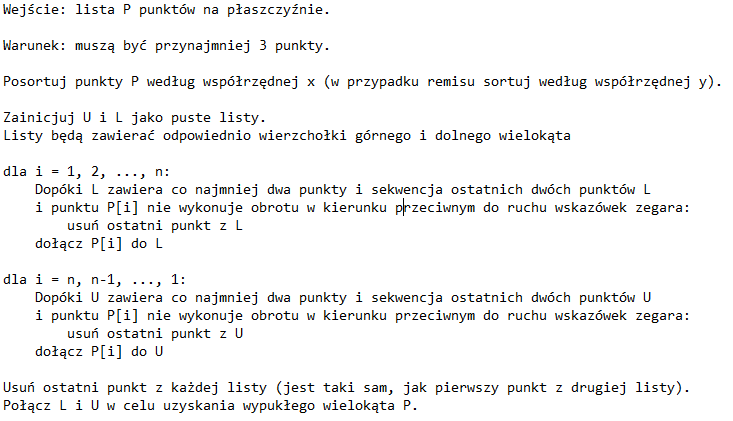
\includegraphics[scale = 0.6]{Monotone.png}
                \caption{Algorytm łańcucha monotonicznego w pseudokodzie.}
            \end{figure}
    
        \item[II.] Wyszukiwanie w drzewie czwórkowym (Quadtree).
        
            \vspace{2mm}
            Zostanie on wykorzystany do znalezienia najbliższego szpitala z wolnymi miejscami, bezpośrednio po pojawieniu się pacjenta.
            
            \vspace{2mm}
            \qquad Algorytm bazuje na drzewie czwórkowym (Quadtree). Jest to drzewo, którego każdy węzeł może mieć do czterech dzieci. Każdy węzeł drzewa czwórkowego jest powiązany z kwadratem. 
            
            \vspace{2mm}
            Niech:
            
            L - liczba poziomów w drzewie czwórkowym.
            
            $F_{j}$ - zbiór kwadratów na poziomie j drzewa czwórkowego.
            
            $E_{j}$ - zbiór kwadratów zawierający potencjalne najbliższe punkty na poziomie j drzewa czwórkowego.
            
            \vspace{2mm}
            \qquad Algorytm bada $E_{0}, E_{1}$, . . . , $E_{L}$, gdzie $E_{j} \in F_{j}$. Zaczyna od $E_{0} = F_{0}$. Aby wyznaczyć Ej, najpierw oblicza $best_{j - 1}$ - najbliższy punkt q wśród reprezentantów kwadratów w $E_{0} \cup E_{1} \cup$ · · · $\cup$ $E_{j-1}$. Reprezentantem kwadratów jest ostatni wstawiony do danego kwadratu punkt. Następnie sprawdzone zostaje każde dziecko kwadratu w $E_{j-1}$ i dodane do $E_{j}$, pod warunkiem, że odległość q od kwadratu wynosi co najwyżej d(q, $best_{j - 1}$).
            
            \begin{figure}[ht]
                \centering
                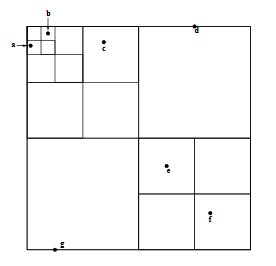
\includegraphics[scale=1]{Quadtree.png}
                \caption{Przykład drzewa czwórkowego.}
            \end{figure}
        
        \item[III.] Algorytm Dijkstry.
        
            \vspace{2mm}
            Zostanie on wykorzystany do znalezienia najbliższego szpitala z wolnymi miejscami w przypadku, gdy pierwszy znaleziony szpital nie posiada wolnych miejsc.
            
            \begin{figure}[ht]
                \centering
                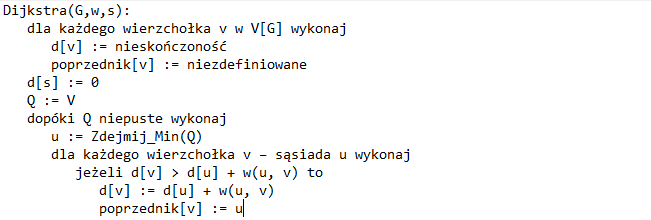
\includegraphics[scale=0.7]{Dijkstra.png}
                \caption{Algorytm Dijkstry w pseudokodzie.}
            \end{figure}
        
    \end{itemize}

\section{Scenariusz działania programu}

    Program będzie wykonywał następujące kroki podczas swojego działania:
    \begin{itemize}
        \item[I.] Wczytanie danych wejściowych.
        \item[II.] Sprawdzenie poprawności otrzymanych danych.
        \item[III.] Stworzenie obszaru "kraju"  zdefiniowanego przez szpitale i obiekty.
        \item[IV.] Dostarczenie pacjentów do szpitali poprzez:
        \begin{itemize}
            \item[a).] Sprawdzenie, czy pacjent znajduje się na terenie kraju.
            \item[b).] Jeżeli tak, to dostarczenie go do najbliższego szpitala.
            \item[c).] Jeśli wybrany w poprzednim kroku szpital nie posiada wolnych łóżek, to znalezienie najbliższego szpitala, który mógłby przyjąć pacjenta i dostarczenie go tam. 
        \end{itemize}
        \item[V.] Wyświetlenie animacji dostarczania pacjentów wraz z informacjami o dokonywanych czynnościach.
    \end{itemize}
    
\section{Testowanie}

    \subsection{Używane narzędzia i opis testów}
    
        Testy programu zostaną napisane we frameworku TestNG. Ich nazwy będą zgodne z ustaloną konwencją nazewniczą (punkt 6.2).
        
        \vspace{4mm}
        Napisane testy będą głównie skupiały się na sprawdzeniu poprawności zaimplementowanego przez nasz zespół algorytmu. Dokładnie zostanie przetestowana również poprawność czytania danych z plików i dodawania pacjentów. Graficzny interfejs użytkownika zostanie przetestowany manualnie przez członków naszego zespołu.\\
        Przygotowane testy skupią się również na możliwych warunkach brzegowych:
        
        \begin{itemize}
            \item Błędny format pliku wejściowego
            \item Błędna struktura pliku wejściowego
            \item Niepoprawne dane w pliku wejściowym
            \item Pusty plik wejściowy
            \item Plik wejściowy zawierający dane przekraczające dopuszczalny zakres\\ przyjmowany przez program
        \end{itemize}
    
        \subsection{Konwencja nazewnicza}
        
        Nazwy testów będą zgodne z następującą konwencją nazewniczą:
        
        \vspace{2mm}
        
        \textbf{nazwaMetody\_testowaneZachowanie\_spodziewaneZachowanie}
\end{document}